\documentclass{article}
\usepackage{graphicx} % Required for inserting images
\usepackage{amsmath}
\usepackage{amsfonts}
\usepackage[margin=2.5cm]{geometry}

\title{CS229 - Problem Set 2}
\author{Or Haifler}
\date{November 2023}

\begin{document}

\maketitle

\section*{Exercise 2}
\subsection*{(a)}

\begin{align*}
    & \frac{\partial}{\partial\theta_{0}}\ell(\theta)=\sum_{i=1}^{m}\frac{\partial}{\partial\theta_{0}}\log h_{\theta}(x^{(i)})^{y^{(i)}}(1-h_{\theta}(x^{(i)}))^{1-y^{(i)}}=y^{(i)}\sum_{i=1}^{m}\frac{\partial}{\partial\theta_{0}}\log h_{\theta}(x^{(i)})+(1-y^{(i)})\sum_{i=1}^{m}\frac{\partial}{\partial\theta_{0}}\log(1-h_{\theta}(x^{(i)})) \\
    & =y^{(i)}\sum_{i=1}^{m}(1-h_{\theta}(x^{(i)}))x_{0}^{(i)}-(1-y^{(i)})\sum_{i=1}^{m}h_{\theta}(x^{(i)})x_{0}^{(i)}=\sum_{i=1}^{m}(y^{(i)}-h_{\theta}(x^{(i)}))x_{0}^{(i)}=\sum_{i=1}^{m}(y^{(i)}-h_{\theta}(x^{(i)}))                                                                                                                             \\
    & \frac{\partial}{\partial\theta_{0}}\ell(\theta)=0\implies\sum_{i=1}^{m}(y^{(i)}-h_{\theta}(x^{(i)}))=0\implies\sum_{i=1}^{m}\mathbb{I}{y^{(i)}=1}=\sum_{i=1}^{m}p(y^{(i)}=1|x^{(i)};\theta)                                                                                                                                                     \\
    & \implies\frac{\sum_{i=1}^{m}\mathbb{I}{y^{(i)}=1}}{|{i\in I_{a,b}}|}=\frac{\sum_{i=1}^{m}p(y^{(i)}=1|x^{(i)};\theta)}{|{i\in I_{a,b}}|}
\end{align*}

\subsection*{(b)}
Both statements aren't true, suppose $(a,b)=(0.5,1)$, then if the model achieves perfect score we get $\sum_{i=1}^m \mathbb{I}\{y^{(i)}=1\}=|\{i\in I_{a,b}\}|$, but $0.5 < p(y^{(i)}|x^{(i)};\theta) < 1$, and thus $\frac{\sum_{i=1}^{m}p(y^{(i)}=1|x^{(i)};\theta)}{|{i\in I_{a,b}}|}<\frac{\sum_{i=1}^{m}\mathbb{I}{y^{(i)}=1}}{|{i\in I_{a,b}}|}$, so the model isn't perfectly calibrated.

\subsection*{(c)}
If we'll use $L_{2}$ regularization(with $\lambda\not = 0$), the loss function will be $$J(\theta)=\sum_{i=1}^{m}y^{(i)}\log h_{\theta}(x^{(i)})+\sum_{i=1}^{m}(1-y^{(i)})\log(1-h_{\theta}(x^{(i)}))+\frac{\lambda}{2}\|\theta\|_{2}^{2}$$
And the learned parameter will be different, because
$$\frac{\partial}{\partial\theta_{0}}\ell(\theta)=0\implies\sum_{i=1}^{m}(y^{(i)}-h_{\theta}(x^{(i)}))+\lambda\theta_{0}=0\implies\sum_{i=1}^{m}1{y^{(i)}=1}=\sum_{i=1}^{m}p(y^{(i)}=1|x^{(i)};\theta)+\lambda\theta_{0}$$
And we got $\sum_{i=1}^{m}1{y^{(i)}=1}\not = \sum_{i=1}^{m}p(y^{(i)}=1|x^{(i)};\theta)$

\newpage

\section*{Exercise 3}
\subsection*{(a)}
\begin{align*}
  \theta_{MAP}=\underset{\theta}{\arg\max}p(\theta|x,y)=\underset{\theta}{\arg\max}\frac{p(\theta,x,y)}{p(x,y)}=\underset{\theta}{\arg\max}\frac{p(y|x,\theta)p(x,\theta)}{p(x,y)}=\underset{\theta}{\arg\max}\frac{p(y|x,\theta)p(\theta)p(x)}{p(x,y)}=\underset{\theta}{\arg\max}p(y|x,\theta)p(\theta)
\end{align*}
\subsection*{(b)}
\begin{align*}
    & \theta_{MAP}=\underset{\theta}{\arg\max}p(y|x,\theta)p(\theta)=\underset{\theta}{\arg\max}\log p(y|x,\theta)p(\theta)=\underset{\theta}{\arg\max}\log p(y|x,\theta)+\log p(\theta)              \\
    & =\underset{\theta}{\arg\min}(-\log p(y|x,\theta)-\log p(\theta))                                                                                                                                \\
    & p(\theta)=\frac{1}{(2\pi)^{n/2}\eta^{n}}\exp\Big(-\frac{1}{2\eta^{2}}\theta^{T}\theta\Big)=\frac{1}{(2\pi)^{n/2}\eta^{n}}\exp\Big(-\frac{1}{2\eta^{2}}\|\theta\|_{2}^{2}\Big)                   \\
    & \theta_{MAP}=\underset{\theta}{\arg\min}(-\log p(y|x,\theta)-\log p(\theta))=\underset{\theta}{\arg\min}(-\log p(y|x,\theta)+\frac{1}{2\eta^{2}}\|\theta\|_{2}^{2}),\lambda=\frac{1}{2\eta^{2}}
\end{align*}

\subsection*{(c)}
\begin{align*}
    & p(y^{(i)}|x^{(i)},\theta)=\frac{1}{\sqrt{2\pi}\sigma}\exp\Big(-\frac{1}{2\sigma^{2}}(y^{(i)}-\theta^{T}x^{(i)})^{2}\Big)                                                                                    \\
    & p(Y|X,\theta)=\prod_{i=1}^{m}p(y^{(i)}|x^{(i)},\theta)=\prod_{i=1}^{m}\frac{1}{\sqrt{2\pi}\sigma}\exp\Big(-\frac{1}{2\sigma^{2}}(y^{(i)}-\theta^{T}x^{(i)})^{2}\Big)                                        \\
    & \frac{1}{(2\pi)^{m/2}\sigma^{m}}\exp\Big(-\frac{1}{2\sigma^{2}}\sum_{i=1}^{m}(y^{(i)}-\theta^{T}x^{(i)})^{2}\Big)=\frac{1}{(2\pi)^{m/2}\sigma^{m}}\exp\Big(-\frac{1}{2\sigma^{2}}\|Y-X\theta\|_{2}^{2}\Big) \\
    & \log p(Y|X,\theta)=\lambda-\frac{1}{2\sigma^{2}}\|Y-X\theta\|_{2}^{2},\lambda=-\frac{m}{2}\log2\pi-m\log\sigma                                                                                              \\
    & \theta_{MAP}=\underset{\theta}{\arg\min}\frac{1}{2\sigma^{2}}\|Y-X\theta\|_{2}^{2}+\frac{1}{2\eta^{2}}\|\theta\|_{2}^{2}                                                                                    \\
    & J(\theta)=\frac{1}{2\sigma^{2}}\|Y-X\theta\|_{2}^{2}+\frac{1}{2\eta^{2}}\|\theta\|_{2}^{2},\nabla_{\theta}J(\theta)=\frac{1}{\sigma^{2}}(\|X\|_{2}^{2}\theta-X^{T}Y)+\frac{1}{\eta^{2}}\theta=0             \\
    & \theta_{MAP}=\underset{\theta}{\arg\min}J(\theta)=(\|X\|_{2}^{2}+\frac{\sigma^{2}}{\eta^{2}}I)^{-1}X^{T}Y
\end{align*}
\subsection*{(d)}
\begin{align*}
    & p(\theta)=\frac{1}{(2b)^{n}}\exp\Big(-\frac{1}{b}\|\theta\|_{1}\Big),\log p(\theta)=-n\log2b-\frac{1}{b}\|\theta\|_{1}                                                                            \\
    & \theta_{MAP}=\underset{\theta}{\arg\min}\frac{1}{2\sigma^{2}}\|Y-X\theta\|_{2}^{2}-\log p(\theta)=\underset{\theta}{\arg\min}\frac{1}{2\sigma^{2}}\|Y-X\theta\|_{2}^{2}+\frac{1}{b}\|\theta\|_{1} \\
    & J(\theta)=\|Y-X\theta\|_{2}^{2}+\lambda\|\theta\|_{1},\theta_{MAP}=\underset{\theta}{\arg\min}J(\theta),\lambda=\frac{2\sigma^{2}}{b}
\end{align*}

\newpage

\section*{Exercise 4}
\subsection*{(a)}
$K$ is positive semidefinite, because $\langle Kz,z \rangle = \langle (K_{1} + K_{2})z,z \rangle = \langle K_{1}z,z \rangle + \langle K_{2}z,z \rangle \ge 0$

\subsection*{(b)}
$K$ doesn't have to be a kernel, for $K_{1}\succeq 0,K_{2}=2K_{1}\succeq0$ we got $K=-K_{1}\preceq0$

\subsection*{(c)}
$K$ is necessarily a kernel, $\langle Kz,z \rangle = \langle aK_{1}z,z \rangle = a \langle K_{1}z,z \rangle \ge 0$

\subsection*{(d)}
$K$ isn't a kernel, because $\langle Kz,z \rangle = \langle aK_{1}z,z \rangle = a \langle K_{1}z,z \rangle \le 0$

\subsection*{(e)}
We know that there are $\phi,\psi$ such that $K_{1}(x,z)=\phi(x)^T\phi(z),K_{2}(x,z)=\psi(x)^T\psi(z)$, so
\begin{align*}
    & \langle Kz,z\rangle=z^{T}Kz=\sum_{i}\sum_{j}z_{i}K_{ij}z_{j}=\sum_{i}\sum_{j}z_{i}K_{1}(x^{(i)},x^{(j)})K_{2}(x^{(i)},x^{(j)})z_{j}                                                                   \\
    & \sum_{i}\sum_{j}z_{i}\phi(x^{(i)})^{T}\phi(x^{(j)})\psi(x^{(i)})^{T}\psi(x^{(j)})z_{j}=\sum_{i}\sum_{j}z_{i}z_{j}\sum_{k}\phi(x^{(i)})_{k}\phi(x^{(j)})_{k}\sum_{l}\psi(x^{(i)})_{l}\psi(x^{(j)})_{l} \\
    & =\sum_{i}\sum_{j}\sum_{k}\sum_{l}z_{i}z_{j}\phi(x^{(i)})_{k}\phi(x^{(j)})_{k}\psi(x^{(i)})_{l}\psi(x^{(j)})_{l}=\sum_{k}\sum_{l}\sum_{i}[z_{i}\phi(x^{(i)})_{k}\psi(x^{(i)})_{l}]^{2}\ge0
\end{align*}

\subsection*{(f)}
$\langle Kz,z \rangle = \sum_{i=1}^{n}\sum_{j=1}^{n}z_{i}z_{j}f(x^(i))f(x^(j))=[z^Tf_{x}]^2 \ge 0, f_{x}=\begin{bmatrix}
    f(x^{(1)}) \\
    f(x^{(2)}) \\
    \vdots     \\
    f(x^{(n)})
  \end{bmatrix}$

\subsection*{(g)}
$K$ is a kernel, we know that $K_{3_{ij}}=K_{3}(x^{(i)},x^{(j)})$ is positive semidefinite for $x^{(i)} \in \mathbb{R}^{n}$, and thus $K_{ij}=K_{3}(\phi(x^{(i)}),\phi(x^{(j)})) \succeq 0$

\subsection*{(h)}
Using (a) and (c) and (e) we conclude that for $a,b \ge 0$, $aK_{1}^{i} + bK_{1}^{j} \succeq 0$, and hence if we generalize for multiple summands we'll get $K=\sum_{i=1}^{n}\alpha_{i}K_{1}^{i}\succeq 0$

\newpage

\section*{Exercise 5}
\subsection*{(a)}
\subsubsection*{i.}
\begin{align*}
    & \theta^{(0)}=\vec{0}, \theta^{(i)}=\sum_{j=1}^{i}\beta_{j}
  \phi(x^{(j)})
\end{align*}

\subsubsection*{ii.}
\begin{align*}
    & h_{\theta^{(i)}}(\phi(x^{(i+1)}))=g(\theta^{(i)^{T}}\phi(x^{(i+1)}))=\text{sign}(\theta^{(i)^{T}}\phi(x^{(i+1)}))=\text{sign}\Big(\sum_{j=1}^{i}\beta_{j}\phi(x^{(j)})^{T}\phi(x^{(i+1)})\Big) \\
    & =\text{sign}\Big(\sum_{j=1}^{i}\beta_{j}\langle\phi(x^{(j)}),\phi(x^{(i+1)})\rangle\Big)=\text{sign}\Big(\sum_{j=1}^{i}\beta_{j}K(x^{(j)},x^{(i+1)})\Big)
\end{align*}

\subsubsection*{iii.}
\begin{align*}
    & \theta^{(i+1)}:=\theta^{(i)}+\alpha\Big(y^{(i+1)}-h_{\theta^{(i)}}(\phi(x^{(i+1)}))\Big)\phi(x^{(i+1)})=\sum_{j=1}^{i}\beta_{j}\phi(x^{(j)})+\alpha\Big(y^{(i+1)}-\text{sing}\Big(\sum_{j=1}^{i}\beta_{j}K(x^{(j)},x^{(i+1)})\Big)\Big)\phi(x^{(i+1)}) \\
    & =\sum_{j=1}^{i+1}\beta_{j}\phi(x^{(j)}),\beta_{i+1}=\alpha\Big(y^{(i+1)}-\text{sing}\Big(\sum_{j=1}^{i}\beta_{j}K(x^{(j)},x^{(i+1)})\Big)\Big)
\end{align*}


\subsection*{(c)}
\begin{figure}
  \centering
  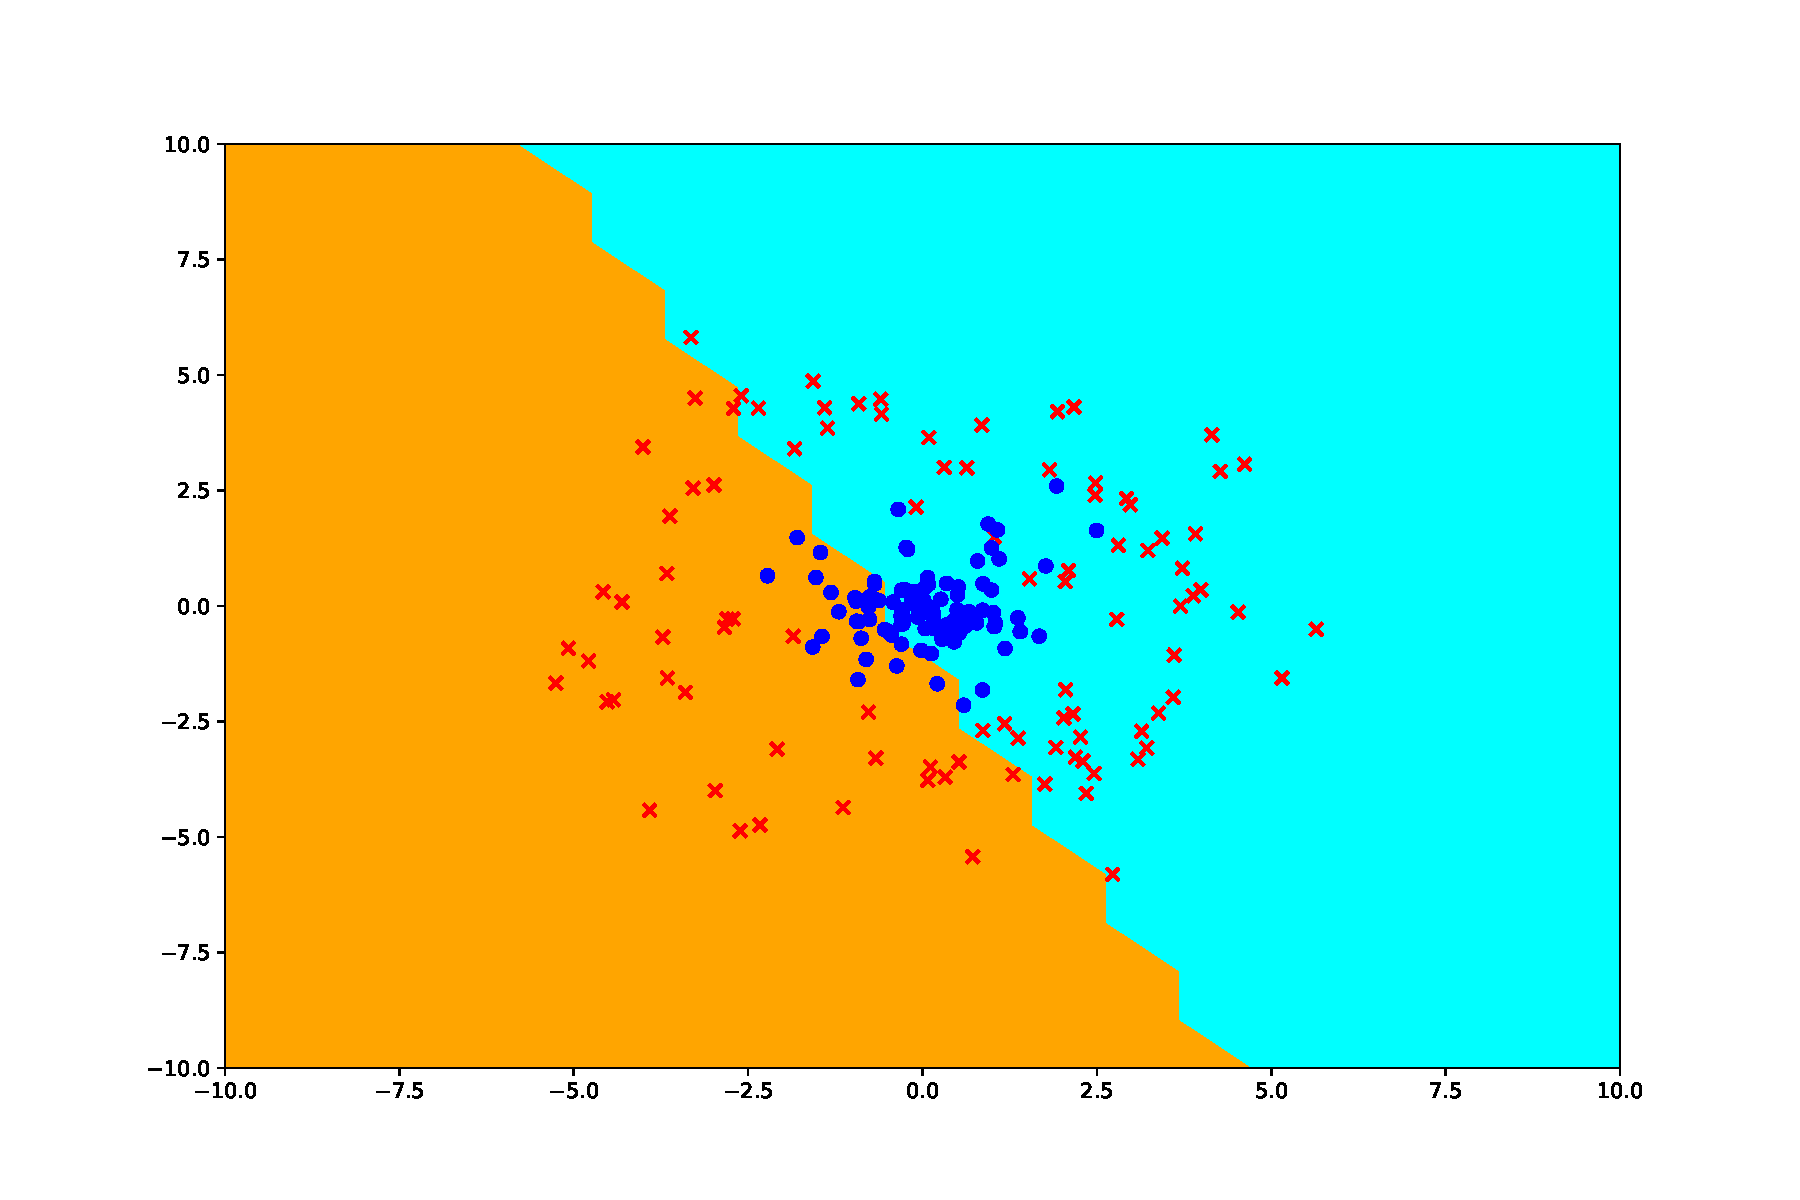
\includegraphics[width=1\textwidth]{images/p05_dot_output.pdf}
  \caption{Dot kernel}
  \label{fig:enter-label}
\end{figure}

\begin{figure}[h]
  \centering
  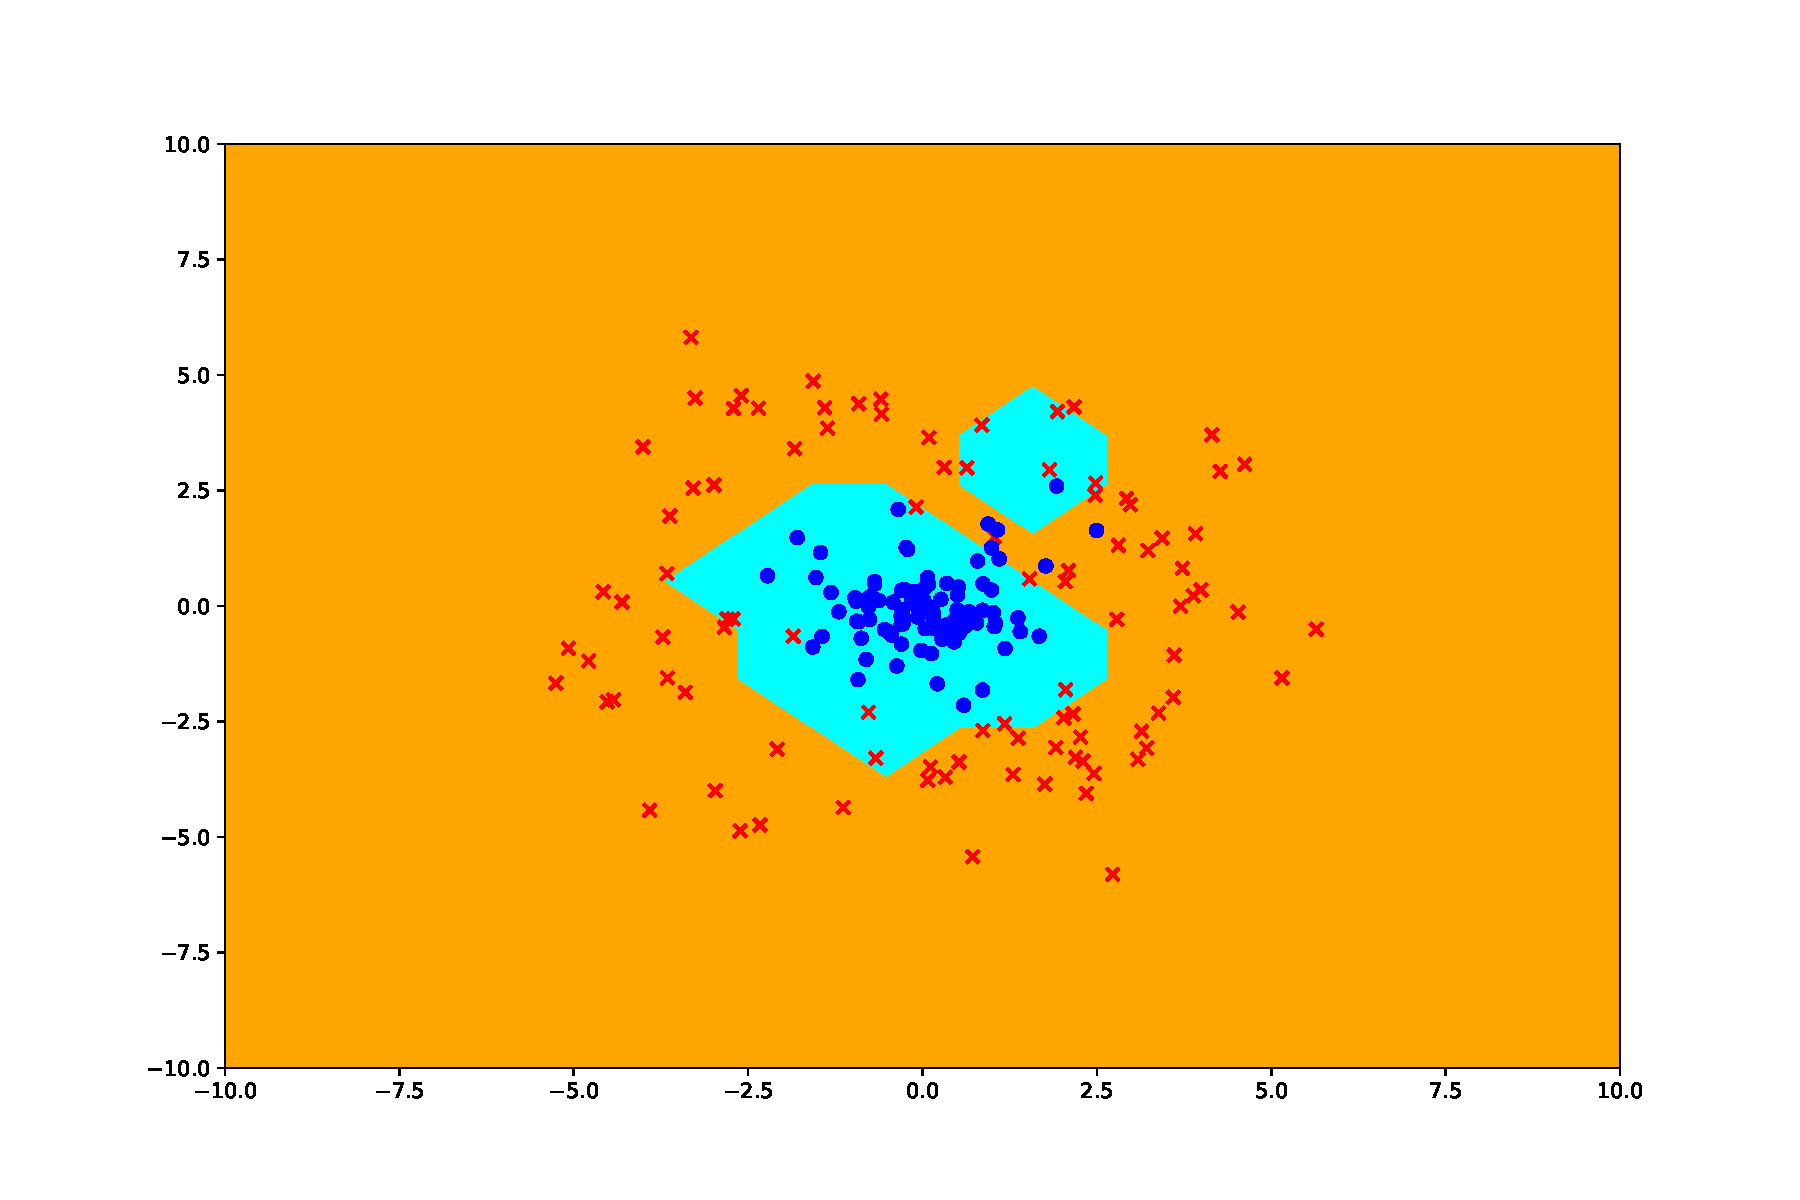
\includegraphics[width=1\textwidth]{images/p05_rbf_output.pdf}
  \caption{RBF kernel}
  \label{fig:enter-label}
\end{figure}

Dot kernel achieves bad accuracy relative to RBF kernel, because it doesn't perform any feature mapping(and thus the model is a linear classifier), and the dataset isn't linearly separable

\end{document}

